\shorthandoff{"}
\chapter{Methodik}
\label{ch:methodik}

\section{Art der Forschung}
\label{ch:methodik:art}
Um die Forschungsfrage der vorliegenden Master-Thesis zu untersuchen, wird eine quantitative Forschungsarbeit in Form eines Experiments durchgeführt. In diesem Kontext wird ein Empfehlungssystem entwickelt, welches sowohl uni- als auch bilaterale Vorschläge zur Besetzung offener Projektpositionen generiert. Für beide Ansätze werden dieselben Projektbeschreibungen und Mitarbeiter als Eingabe verwendet. Die beiden Empfehlungsverfahren unterscheiden sich lediglich in der Art, in welcher sie die vorhandenen Angestellten für die eingegebenen Stellen sortieren. Zur Beantwortung der Forschungsfrage wird eine Fallstudie mit Projektmanagern und -mitarbeitern durchgeführt.

Die Projektmanager erhalten die sortierten Mitarbeiter beider Systeme für vorausgewählte Projektpositionen in Form von Listen. Anschließend bewerten sie auf einer vordefinierten Skala, welche Arbeitsleistung sie von denen in der vorliegenden Reihenfolge dargestellten Mitarbeitern für die jeweiligen Stellen erwarten. Dabei wird evaluiert, ob sie die erwartete Leistung der vorgeschlagenen Angestellten des bilateralen Ansatzes höher bewerten, als die der unilateralen Variante.

Die Mitarbeiter des Unternehmens erhalten Übersichten über die vorausgewählten Projektpositionen. Daraufhin bewerten sie auf einer vordefinierten Skala, wie zufrieden sie mit einer Tätigkeit auf den vorliegenden Projektpositionen wären. Dabei wird überprüft, ob das bilaterale Empfehlungssystem die Angestellten für die Projektpositionen höher positioniert, bei welchen diese eine hohe Zufriedenheit erwarten bzw. niedriger positioniert, wenn diese eine geringe Zufriedenheit prognostizieren.

Im Rahmen der vorliegenden Master-Thesis wird ausschließlich der komplementäre \ac{PEFit} auf Facetten-Ebene betrachtet. Hierbei werden einzig die für offene Projektpositionen benötigten Kompetenzen zur Bestimmung der Kongruenz herangezogen. Weitere Faktoren wie Kundennamen oder Branchen werden nicht berücksichtigt. Im Sinne des ergänzenden \acp{PEFit} wird vorausgesetzt, dass eine grundlegende Übereinstimmung der Werte von Mitarbeitern und Unternehmen bzw. Projekttätigkeiten bereits vor Anstellung der Arbeitnehmer überprüft wurde.

Durchgeführt werden das Experiment und die Fallstudie mit Projektmanagern und Mitarbeitern des Fachbereichs \ac{JES} der EXXETA AG mit Hauptsitz in Karlsruhe. Das Unternehmen ist spezialisiert auf IT-Beratungsleistungen und arbeitet vorrangig projektbasiert. Passende Angestellte zu offenen Projektpositionen zuzuordnen ist in diesem Betrieb dementsprechend eine häufig auftretende Aufgabe.

\section{Vorhandene Daten im Unternehmen}
\label{ch:methodik:versuchsaufbau}
Die Mitarbeiter der EXXETA AG pflegen ihre Kompetenzen in einem Intranet. Dort steht eine Liste mit \anzFaehigkeiten Fähigkeiten wie beispielsweise "Java", "DSGVO" und "Digitale Transformation" zur Verfügung. Diese können die Angestellten über die in Abbildung \ref{fig:methodik:versuchsaufbau:daten:abb1} dargestellte Skala bewerten.

\begin{figure}[h]
	\centering
	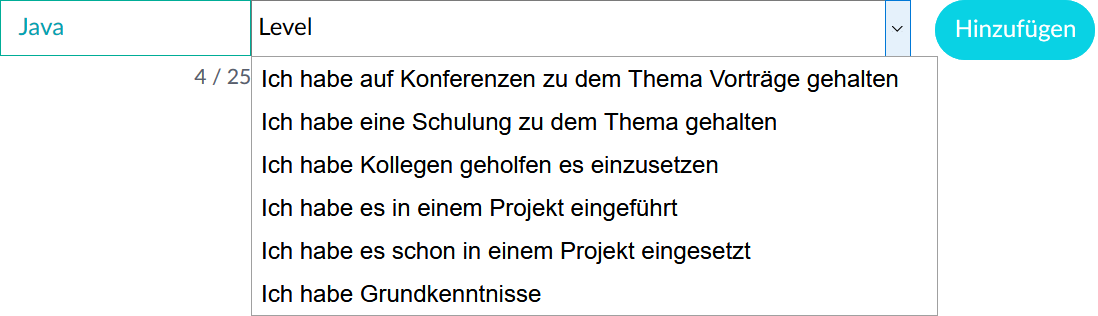
\includegraphics[width=1\textwidth]{gfx/skill-level.png}
	\caption{Hinzufügen einer Fähigkeit mit Angabe des entsprechenden Kenntnisniveaus im EXXETA-Intranet}
	\label{fig:methodik:versuchsaufbau:daten:abb1}
\end{figure}

Die Abstufungen in Abbildung \ref{fig:methodik:versuchsaufbau:daten:abb1} werden beim Speichern in ganzzahlige Werte von 0 ("Ich habe Grundkenntnisse") bis fünf ("Ich habe auf Konferenzen zu dem Thema Vorträge gehalten") übertragen.

Aufgrund der klaren Beschreibungen der einzelnen Stufen in Abbildung \ref{fig:methodik:versuchsaufbau:daten:abb1} kann der in Kapitel \ref{ch:empfehlungssysteme:cf:speicherbasiert} angesprochene Bias bei der Selbsteinschätzung weitgehend ausgeschlossen werden. Außerdem ist es in der vorliegenden Problemstellung gut möglich, dass einzelne Mitarbeiter ihre Kompetenzen bewusst besser oder schlechter bewerten als andere Kollegen. Dieser Sachverhalt ist insbesondere auf längere Berufserfahrung zurückzuführen. Aus diesen Gründen wird bei der Empfehlungsbestimmung auf eine Mittelwert-Zentrierung verzichtet.

Damit Projektmanager Vorschläge erhalten können, müssen sie die für offene Projektpositionen nachgefragten Fähigkeiten mitsamt der benötigten Kenntnisniveaus festlegen. Die relevanten Kompetenzen bestimmen die Verantwortlichen in der Regel anhand eingehender Projektanfragen, welche Kunden in unstrukturierter Form, beispielsweise über Telefon oder E-Mail, einreichen. Derartige Anfragen werden täglich in großer Anzahl bearbeitet. Daher wird es für den praktischen Einsatz als sehr umständlich bewertet, wenn Verantwortliche für jede Projektanfrage sämtliche Fähigkeiten auf der sechsstufigen Skala bewerten müssen. Aus diesem Grund werden die Kompetenzniveaus aus Abbildung \ref{fig:methodik:versuchsaufbau:daten:abb1} zur Spezifikation ooffener Projektpositionen auf die Abstufungen "Grundkenntnisse" und "Fortgeschritten" vereinfacht. "Grundkenntnisse" entspricht dabei den ersten drei Stufen und "Fortgeschritten" den oberen drei Fähigkeitsniveaus in Abbildung \ref{fig:methodik:versuchsaufbau:daten:abb1}. Die Priorisierung der Kompetenzen über diese Abstufungen wird gemäß Kapitel \ref{ch:personEnvironmentFit:wichtigkeiten} als Ausdruck von Wichtigkeiten seitens der Projektmanager betrachtet.

Die EXXETA AG erhebt keine Präferenzen der Mitarbeiter bezüglich ihrer Kompetenzen. Um deren Wünsche ebenfalls in die Empfehlungsprozess einzubeziehen, wird im Rahmen dieser Thesis eine Umfrage durchgeführt. Die Angestellten des Bereichs \acl{JES} erhalten zu diesem Zweck einen Fragebogen mit den \anzFaehigkeiten im Intranet hinterlegten Fähigkeiten. Dabei werden sie gebeten, sämtliche Kompetenzen auszuwählen, welche sie gerne in einem Projekt anwenden möchten. Ein Auszug aus dem Fragebogen ist in Abbildung \ref{fig:methodik:versuchsaufbau:abb1} dargestellt.

\begin{figure}[h]
	\centering
	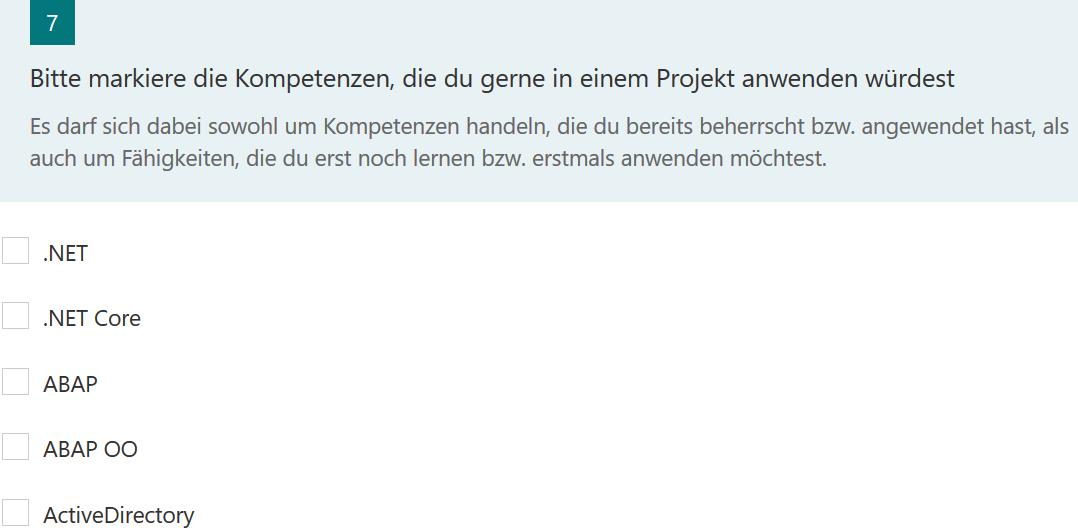
\includegraphics[width=1\textwidth]{gfx/Umfage_Faehigkeiten.png}
	\caption{Auszug aus der Umfrage zur Erhebung der Mitarbeiter-Präferenzen}
	\label{fig:methodik:versuchsaufbau:abb1}
\end{figure}

Die Kompetenzbewertungen der Mitarbeiter und deren Präferenzen dienen im Experiment als Grundlage für ein hybrides Empfehlungssystem.

\section{Verwendetes Empfehlungsverfahren}
\label{ch:methodik:empfehlungsmethode}
Das im Rahmen dieser Master-Thesis implementierte Empfehlungssystem basiert auf der Datenstruktur eines Graphen. Dabei werden die Mitarbeiter der EXXETA AG und deren Fähigkeiten in Form von Knoten dargestellt. Um das Sparsity Problem zu lösen, wird der speicherbasierte Algorithmus von Katz aus Kapitel \ref{ch:empfehlungssysteme:cf:speicherbasiert} angewendet. Da die Anwendung auch über die Master-Thesis hinaus im Unternehmen zum Einsatz kommen soll, ist insbesondere die Langlebigkeit des Verfahrens vorteilhaft gegenüber modellbasierten Methoden. Sollten sich nach Durchführung des Experiments Daten im Unternehmen verändern oder neue Kompetenzen im Intranet hinzugefügt werden, ist das Empfehlungssystem weiterhin ohne zusätzlichen manuellen Aufwand im Betrieb anwendbar. Die hohe algorithmische Komplexität des Katz-Algorithmus ist für die vorliegende Problemstellung tolerierbar, da sich zum Zeitpunkt des Experiments weniger als 1.000 Mitarbeiter im Unternehmen befinden.

Wie in Kapitel \ref{ch:empfehlungssysteme:cf:speicherbasiert} beschrieben, sorgt der Algorithmus von Katz für eine feingranulare Anpassung vorhandener Beurteilungen. Dass Bewertungen von Mitarbeitern gänzlich fehlen, kann bei er EXXETA AG weitgehend ausgeschlossen werden. Führungskräfte fordern ihre Angestellten regelmäßig dazu auf, ihre Kompetenzen im Intranet aktuell zu halten und diese beispielsweise im Rahmen des Mitarbeiter-Jahresgespräches zu pflegen. Angestellte ohne Bewertungen sind folglich nur in Ausnahmefällen zu erwarten. Hierzu zählen beispielsweise Werkstudenten und neue Mitarbeiter.

Um Kaltstarts auch in solchen Ausnahmefällen vorzubeugen, werden zusätzlich zu den Fähigkeiten der Mitarbeiter auch deren Teamzuordnungen in Form eines hybriden Ansatzes beachtet. Dieses Vorgehen hat zusätzlich den Vorteil, dass die Kompetenzen der Mitarbeiter bei Berechnung des Algorithmus feingranular besser bewertet werden, wenn deren direkte Kollegen ähnliche Fähigkeiten beherrschen. Dieses Vorgehen ist im Falle der EXXETA AG als sinnvoll zu bewerten, da dort stets Mitarbeiter mit vergleichbarem fachlichem Hintergrund in einem Team tätig sind. Auch der Manager des Teams ist eine fachliche Führungskraft, dessen Fähigkeiten weitgehend repräsentativ für seine Mitarbeiter sind.%Seine Kompetenzen sind in der Regel jedoch stärker ausgeprägt.

Die Bewertungen der Fähigkeiten und die Teamzuordnungen können für alle Mitarbeiter der EXXETA AG über eine REST-Schnittstelle in Form von JSON aus dem Intranet abgefragt werden. Einzelne Mitarbeiter sind dabei eindeutig über ihre E-Mail-Adresse identifizierbar.

In der vorliegenden Problemstellung werden nicht die Daten aller Angestellten des Unternehmens verwendet. Es wird ausschließlich auf Informationen über Mitarbeiter zurückgegriffen, welche im Rahmen der Befragung Präferenzen spezifiziert haben. Aus diesem Grund wird die REST-Schnittstelle des Intranets im Rahmen der vorliegenden Master-Thesis 

\section{Systemarchitektur}
\label{ch:methodik:versuchsaufbau:systemarchitektur}
Abbildung \ref{fig:methodik:systemarchitekturn:abb1} zeigt die im Rahmen dieser Master-Thesis implementierte Systemarchitektur des Empfehlungssystems.

\begin{figure}[h]
	\centering
	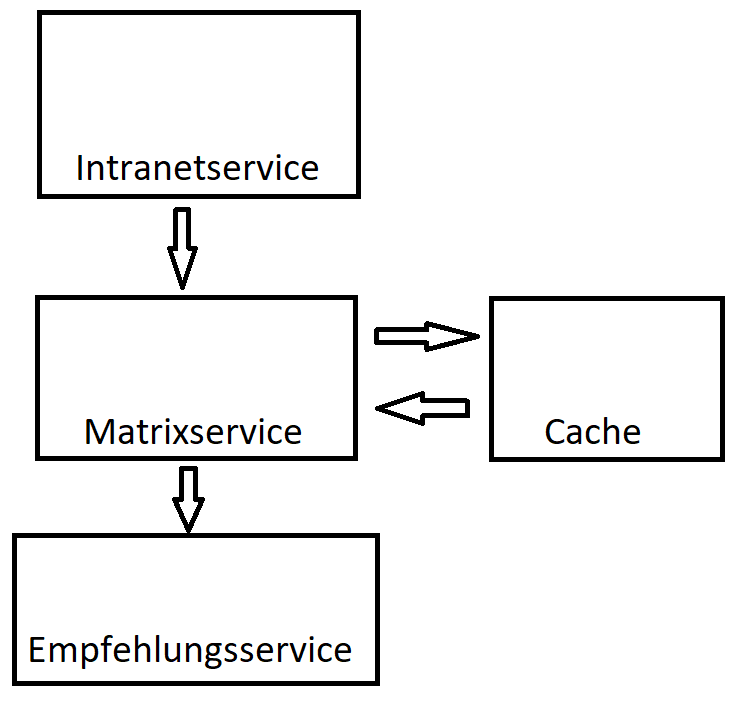
\includegraphics[width=0.75\textwidth]{gfx/Systemarchitektur.png}
	\caption{Systemarchitektur des Empfehlungssystems}
	\label{fig:methodik:systemarchitekturn:abb1}
\end{figure}

Im folgenden werden die einzelnen Komponenten der Anwendung erläutert.

\subsection{Grundlegender Algorithmus}
\label{ch:methodik:versuchsaufbau:grundlegend}



Wie bereits im Kontext von Abbildung \ref{fig:methodik:versuchsaufbau:daten:abb1} erläutert, sind die Bewertungen der Kompetenzen im JSON aus Listing \ref{qc:methodik:versuchsaufbau:daten:qc1} um eins niedriger als in Tabelle \ref{tbl:empfehlungssysteme:arbeitsweise:tbl1}.

Vor Überführung der Daten der REST-Schnittstelle in die Datenstruktur eines Graphen, werden die sechsstufigen Beurteilungen der Fähigkeiten der Mitarbeiter auf die zweistufige Skala der Projektmanager angepasst. Hierbei werden Bewertungen auf dem Niveau "Grundkenntnisse" auf ein Kantengewicht von \kantengewichtString und "fortgeschrittene" Beurteilungen auf \kantengewichtHochString vereinfacht. Diese Werte entsprechen den höchstmöglichen Bewertungen auf dem jeweiligen Kompetenzniveau. Ein Gewicht von 0 symbolisiert ausschließlich nicht bewertete Fähigkeiten.

Um eine weitere Erhöhung der Komplexität des Algorithmus von Katz zu vermeiden, werden die Teams nicht als zusätzliche Knoten in den Graphen eingefügt. Die Beziehungen werden stattdessen über direkte Kanten zwischen Kollegen dargestellt. Das Kantengewicht zwischen zwei Teammitgliedern bzw. einem Angestellten zu seinem Manager wird auf \teamgewichtString festgelegt. Dieser Wert wird verwendet, um die Teamzugehörigkeit schwach in die Berechnung mit einzubeziehen, die individuellen Beurteilungen der Mitarbeiter jedoch höher zu gewichten.%Über diesen Ansatz sind alle Teammitglieder schwach miteinander verbunden, sodass die vorhandenen Bewertungen wenig verzerrt werden und dennoch auch im Fall eines Kaltstarts für Mitarbeiter ohne explizite Bewertungen Beurteilungen bestimmt werden können.

Abbildung \ref{fig:methodik:versuchsaufbau:unilateral:abb1} zeigt die Darstellung der Kompetenzen und die Teamzuordnungen der Angestellten aus Tabelle \ref{tbl:empfehlungssysteme:arbeitsweise:tbl1} in der Form eines Graphen.%Außerdem wurde eine offene Projektposition in Form eines Pseudo-Mitarbeiters eingefügt.

\begin{figure}[h]
	\centering	
	\begin{tikzpicture}[node distance={32mm}, thick, main/.style = {draw, circle}] 
		\node[main, fill=itemcolor] (MongoDB) {$MongoDB$}; 
		\node[main, fill=itemcolor] (Python) [below right of=MongoDB] {$Python$}; 
		\node[main, fill=itemcolor] (MySQL) [above right of=Python] {$MySQL$}; 
		\node[main, fill=itemcolor] (Java) [below right of=MySQL] {$Java$}; 
		\node[main, fill=itemcolor] (HDFS) [above right of=Java] {$HDFS$}; 
		\node[main, fill=itemcolor] (Spark) [below right of=HDFS] {$Spark$};
		
		\node[main, fill=usercolor] (Jane) [above right of=MongoDB] {$Jane D.$}; 
		\node[main, fill=usercolor] (John) [above left of=HDFS] {$John D.$}; 
		\node[main, fill=usercolor] (Max) [below of=MySQL] {$Max M.$};
		\node[main, fill=usercolor] (Erika) [above right of=HDFS] {$Erika M.$};
		
		\draw (Jane) -- node[midway, right] {\kantengewichtHoch} (Python);
		\draw (Jane) -- node[midway, above] {\kantengewicht} (MySQL);
		\draw (Jane) -- node[midway, above] {\kantengewicht} (MongoDB);
		
		\draw (John) -- node[midway, right] {\kantengewicht} (HDFS);		
		\draw (John) -- node[midway, right] {\kantengewicht} (Java);
		\draw (John) -- node[midway, above] {\kantengewicht} (MySQL);
		
		\draw (Erika) -- node[midway, above] {\kantengewichtHoch} (HDFS);
		\draw (Erika) -- node[midway, right] {\kantengewicht} (Spark);
		
		\draw (Max) -- node[midway, above] {\kantengewicht} (Java);
		\draw (Max) -- node[midway, above] {\kantengewicht} (Python);
		\draw (Max) -- node[midway, right] {\kantengewicht} (MySQL);
		
		%\draw (Jane) -- node[midway, above] {\kantengewicht} (John);
		\draw (Jane) -- node[midway, left] {\teamgewicht} (Max);
		%\path (Jane) edge[bend left=25] node[midway, above] {\kantengewicht} (Erika);
		
		%\draw (John) -- node[midway, right] {\kantengewicht} (Max);
		\draw (John) -- node[midway, above] {\teamgewicht} (Erika);
		
		%\path (Max) edge[bend right=40] node[midway, above] {\kantengewicht} (Erika);
		
		%\node[main, fill=usercolor] (Projekt) [below of=Java] {$Projekt$}; 
		%\path (Projekt) edge[bend left=40] node[midway, above] {\kantengewicht} (MongoDB);
		%\path (Projekt) edge[bend right=25] node[midway, above] {\kantengewicht} (Spark);
		%\draw (Projekt) -- node[midway, right] {\kantengewichtHoch} (Java);
	\end{tikzpicture}
	
	\caption{Graph aus Abbildung \ref{fig:empfehlungssysteme:cf:speicherbasiert:abb2} mit zusätzlicher Teamzuordnung und offener Projektposition}
	\label{fig:methodik:versuchsaufbau:unilateral:abb1}
\end{figure}

Die Daten des Graphen aus Abbildung \ref{fig:methodik:versuchsaufbau:unilateral:abb1} dienen als Grundlage zur Berechnung des Katz-Algorithmus anhand von Gleichung \ref{frml:empfehlungssysteme:cf:speicherbasiert:formel4}. Dabei wird der Wert von $\beta$ über folgende Gleichung \ref{frml:methodik:versuchsaufbau:grundlegend:formel1} bestimmt: 
\begin{equation}
	\beta = \frac{1/\lambda}{\nenner}
	\label{frml:methodik:versuchsaufbau:grundlegend:formel1}
\end{equation}
Durch das in in Gleichung \ref{frml:methodik:versuchsaufbau:grundlegend:formel1} dargestellte Vorgehen ist sichergestellt, dass $\beta$ auch bei sich ändernder Datenlage stets kleiner als $1/\lambda$ ist. Wie in Kapitel \ref{ch:empfehlungssysteme:cf:speicherbasiert} dargelegt, entspricht $\lambda$ dem größten Eigenwert der Adjazenzmatrix des Graphen. Aufgrund der Division durch \nenner ist $\beta$ stets so groß, dass von einem Zielknoten weit entfernte Knoten noch in die Berechnung einbezogen werden, nahe Knoten jedoch stärker gewichtet werden. Auf diese Weise erhalten die Knoten ein höheres Gewicht in der Berechnung, welche mit den direkten Teamkollegen bzw. den unmittelbar beherrschten Kompetenzen eines Zielnutzers in Verbindung stehen.

Zur effizienteren Vorschlagsbestimmung wird die Ergebnismatrix zwischengespeichert. Somit muss die algorithmisch komplexe Berechnung des Katz-Algorithmus nur ausgeführt werden, wenn sich Daten im Unternehmen ändern. Dieses Vorgehen ermöglicht es, immer die aktuellen Daten des Unternehmens bei der Empfehlungsberechnung zu betrachten und gleichzeitig eine zu modellbasierten Verfahren vergleichbare Effizienz zu erreichen.

Die Bestimmung der Empfehlungen anhand der zwischengespeicherten Matrix erfolgt in zwei separaten Empfehlungskomponenten. Eine der beiden Module verfolgt einen unilateralen, die andere einen bilateralen Ansatz. Beide Module unterscheiden sich ausschließlich in der Art, wie sie die Mitarbeiter sortieren.

\subsection{Unilateraler Empfehlungsansatz}
\label{ch:methodik:versuchsaufbau:unilateral}
Die unilaterale Empfehlungskomponente fokussiert bei der Bestimmung von Vorschlägen ausschließlich die Präferenzen des Projektmanagers. Im Sinne des \acp{PEFit} wird folglich nur die Anforderungen-Fähigkeiten Kongruenz betrachtet.

Wie in Kapitel \ref{ch:empfehlungssysteme:cf:speicherbasiert} beschrieben, ändern sich bei Berechnung des Verfahrens von Katz die Kompetenzbewertungen. Somit es ist nicht ohne Weiteres möglich, die Eingaben eines Projektmanagers mit den Werten in der Ergebnis-Matrix zu vergleichen.

Allerdings befinden sich die Beurteilungen, welche ursprünglich einem gemeinsamen Kompetenzniveau entsprachen, auch nach Berechnung des Algorithmus auf einem vergleichbaren Niveau. Die Werte innerhalb eines Kompetenzbereichs sind lediglich feingranular unterschiedlich. Dieses Phänomen ist in Tabelle \ref{tbl:methodik:versuchsaufbau:unilateral:tbl1} zu beobachten. Dort sind die Bewertungen der Fähigkeit MySQL aus Abbildung \ref{fig:methodik:versuchsaufbau:unilateral:abb1} vor und nach der Berechnung des Katz-Algorithmus eingetragen. Gleiche Kompetenzniveaus sind in der Tabelle durch einheitliche Hintergrundfarben gekennzeichnet.

\begin{table}[h]
	\centering
	\begin{tabular}{c|c|c|c}
		Name & Kompetenzniveau & Wert & Ergebnis \\
		\hline
		 \rowcolor{exxetagray}Erika M. & Keine Kenntnisse & 0                  & 0.565\\
		\hline
		\rowcolor{itemcolor}John D.    & Grundkenntnisse  & \kantengewicht     & 1.202\\
		\rowcolor{itemcolor}Max M.     & Grundkenntnisse  & \kantengewicht     & 1.623\\
		\rowcolor{itemcolor}Jane D.    & Grundkenntnisse  & \kantengewicht     & 1.996
	\end{tabular}
	\caption{Ergebnisse des Katz-Algorithmus für die Kompetenz MySQL im Graphen aus Abbildung \ref{fig:methodik:versuchsaufbau:unilateral:abb1}}
	\label{tbl:methodik:versuchsaufbau:unilateral:tbl1}
\end{table}

In Tabelle \ref{tbl:methodik:versuchsaufbau:unilateral:tbl1} ist veranschaulicht, dass sich die Bewertungen der drei Angestellten mit Grundkenntnissen in MySQL auch nach Berechnung des Katz-Algorithmus auf einem vergleichbaren Niveau befinden. Die Beurteilungen sind, wie erwartet, feingranular unterschiedlich. Auch der Abstand zu Erika Muster ist nach wie vor erkennbar.

Wird anhand der Daten aus Tabelle \ref{tbl:methodik:versuchsaufbau:unilateral:tbl1} ein Mitarbeiter mit der Fähigkeit MySQL gesucht, kann folglich der Angestellte mit dem höchsten Wert im gesuchten Kompetenzbereich als geeignetster Kandidat betrachtet werden. Im vorliegenden Beispiel wäre somit Jane Doe die qualifizierteste Mitarbeiterin für die Suche nach einem Angestellten mit Grundkenntnissen im Umgang mit MySQL. Ihre Bewertung dient daher bei der Bestimmung des \acp{PEFit} für das gesuchte Kompetenzniveau in MySQL als Nullpunkt in Abbildung \ref{fig:methodik:versuchsaufbau:unilateral:abb2}.

\begin{figure}[h]
	\centering
	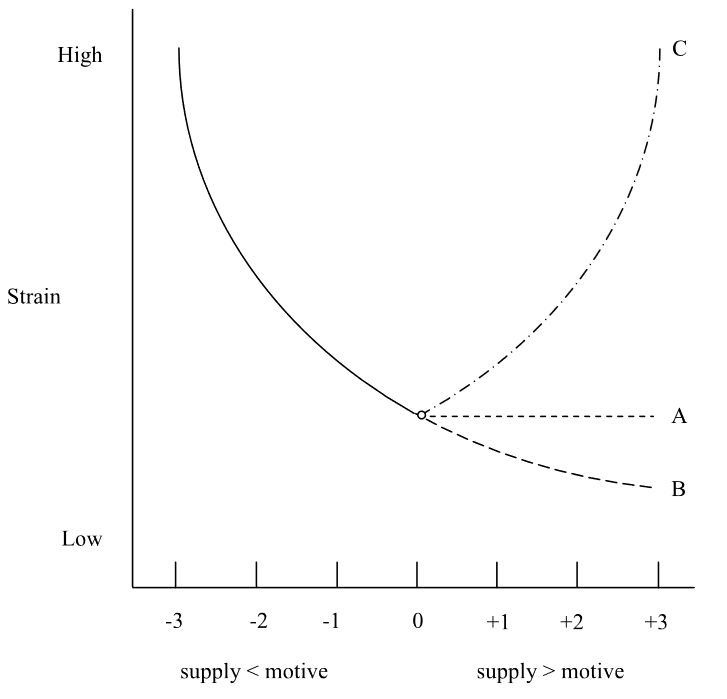
\includegraphics[width=0.75\textwidth]{gfx/ueberschuss_supply_motive.png}
	\caption{Auswirkungen eines Bedürfnisse-Angebote Misfits\\(Eigene Darstellung in Anlehnung an \cite[S. 23]{edwards:2008})}
	\label{fig:methodik:versuchsaufbau:unilateral:abb2}
\end{figure}

Zur Bestimmung des Anforderungen-Fähigkeiten Fits wird angenommen, dass Projektmanager anstreben, offene Projektpositionen mit fachlich optimal passenden Mitarbeitern zu besetzen. Folglich vermeiden sie sowohl eine Über- als auch eine Unterqualifizierung ihrer Angestellten. Aus diesem Grund wird der \ac{PEFit} anhand von Kurve B bestimmt. Dabei wird die quadrierte Differenzberechnung angewendet.

Ist kein Mitarbeiter im gesuchten Kompetenzbereich vorhanden, wird eine Ausnahmebehandlung durchgeführt. Wird nach Grundkenntnissen in einer bestimmten Fähigkeit gesucht und dabei kein passender Kandidat gefunden, wird der wenig qualifizierteste Angestellte auf fortgeschrittenem Niveau als Referenz genutzt. Sucht ein Projektmanager erfolglos nach Mitarbeitern mit fortgeschrittenen Kenntnissen, wird der am Besten qualifizierte Kandidat mit Grundkenntnissen als Referenz verwendet. Sind ausschließlich Mitarbeiter ohne Kenntnisse vorhanden, wird die gesuchte Kompetenz übersprungen, da in diesem Fall kein Mitarbeiter im Graphen mit dieser Fähigkeit verbunden ist und somit alle Kantengewichte 0 sein müssen.

Tabelle \ref{tbl:methodik:versuchsaufbau:unilateral:tbl2} zeigt das Ergebnis einer unilateralen Empfehlungsbestimmung für ein Beispielprojekt mit fortgeschrittenen Kenntnissen in Python und MySQL und Grundkenntnissen in HDFS. Verwendet wurden dabei die Daten des Graphen aus Abbildung \ref{fig:methodik:versuchsaufbau:unilateral:abb1}. Die vollständige Berechnung kann in Anhang \ref{ch:nebenrechnungen:unilateral} nachvollzogen werden.

\begin{table}[h]
	\centering
	\begin{tabular}{c|c|c}
		Positionierung & Mitarbeiter & Abweichung\\
		\hline
		1 & Jane D.  & 0.30\\
		2 & Max M.   & 1.21\\
		3 & John D.  & 4.06\\
		4 & Erika M. & 7.72
	\end{tabular}
	\caption{Ergebnisliste der unilateralen Empfehlungskomponente für die Daten aus Abbildung \ref{fig:methodik:versuchsaufbau:unilateral:abb1}}
	\label{tbl:methodik:versuchsaufbau:unilateral:tbl2}
\end{table}

Ähnlich zum unilateralen Algorithmus arbeitet auch die bilaterale Empfehlungskomponente. Diese bezieht neben dem Anforderungen-Fähigkeiten Fit auch die Präferenzen der Mitarbeiter bzw. die Bedürfnisse-Angebote Kongruenz in die Berechnung mit ein.

\subsection{Bilateraler Empfehlungsansatz}
\label{ch:methodik:versuchsaufbau:bilateral}
Die Präferenzen der Mitarbeiter werden im Unternehmen über eine Befragung erhoben. Zu diesem Zweck erhalten die Angestellten eine Liste mit den Fähigkeiten aus dem Intranet. Auf dieser können sie über einen boolschen Wert für jede Kompetenz festlegen, ob sie diese zukünftig in Projekten anwenden möchten. Sie können dabei sowohl bereits beherrschte Fähigkeiten auswählen, als auch Kompetenzen, welche diese zukünftig erst erlernen bzw. erstmals einsetzen möchten.

Hinsichtlich der Linien aus Abbildung \ref{fig:methodik:versuchsaufbau:unilateral:abb2} wird von den Mitarbeitern erwartet, dass diese Unterforderung im Projekt vermeiden möchten. Daher wird auch in diesem Modul Kurve B über die quadrierte Differenzberechnung implementiert.

Die bilaterale Empfehlungskomponente bezieht die Wünsche der Mitarbeitern in Form von Wichtigkeiten in die Berechnung ein. Wie in Kapitel \ref{ch:personEnvironmentFit:regressionsgleichungen} gefordert, werden hierbei die präferierten Kompetenzen der Angestellten vor der Differenzberechnung mit einem Parameter multipliziert. Die vorliegende Empfehlungskomponente verwendet dabei den Faktor \faktorString. Dieser wird in Anlehnung an die Gewichte der Niveaus Grundkenntnisse (\kantengewichtString) und Fortgeschritten (\kantengewichtHochString) gewählt, welche ebenfalls einer Verdopplung entsprechen. Bei der quadrierten Differenzbestimmung wird somit die folgende Berechnung aus Gleichung \ref{frml:methodik:versuchsaufbau:bilateral:formel1} ausgeführt:
\begin{equation}
	Abweichung = (\faktor * P - E)^2
	\label{frml:methodik:versuchsaufbau:bilateral:formel1}
\end{equation}
Die Multiplikation in Gleichung \ref{frml:methodik:versuchsaufbau:bilateral:formel1} hat zur Folge, dass Mitarbeiter für eine Kompetenz innerhalb ihres beherrschten Niveaus aufsteigen bzw. die untere Grenze des nächst höheren Bereichs erreichen. Sucht ein Projektmanager nach einer Fähigkeit, welche ein Angestellter präferiert, wird dieser bei der Sortierung folglich besser bewertet als bei der unilateralen Variante. Dennoch übertrifft er nicht die geeignetsten Mitarbeiter des nächst höheren Kompetenzniveaus.

Tabelle \ref{tbl:methodik:versuchsaufbau:bilateral:tbl1} zeigt die Anpassungen der Ergebnisse des Katz-Algorithmus durch Angabe von Wichtigkeiten am Beispiel der Fähigkeit MySQL aus Tabelle \ref{tbl:methodik:versuchsaufbau:unilateral:tbl1}.

\begin{table}[h]
	\centering
	\begin{tabular}{c|c|c|c|c}
		Name & Kompetenzniveau & Wert & Präferenz & Erg. uni-/bilateral \\
		\hline
		\rowcolor{exxetagray}Erika M. & Keine Kenntnisse & 0 & wahr & 0.565/1.130\\
		\hline
		\rowcolor{itemcolor}John D. & Grundkenntnisse  & \kantengewicht & falsch & 1.202/1.202 \\
		\rowcolor{itemcolor}Max M. & Grundkenntnisse  & \kantengewicht & wahr & 1.623/3.246\\
		\rowcolor{itemcolor}Jane D. & Grundkenntnisse  & \kantengewicht & falsch & 1.996/1.996
	\end{tabular}
	\caption{Ergebnisse des Katz-Algorithmus für die Kompetenz MySQL im Graphen aus Abbildung \ref{fig:methodik:versuchsaufbau:unilateral:abb1} unter Einbeziehung von Präferenzen}
	\label{tbl:methodik:versuchsaufbau:bilateral:tbl1}
\end{table}

In Tabelle \ref{tbl:methodik:versuchsaufbau:bilateral:tbl1} ist an Erika und Max Muster zu erkennen, dass die Beurteilungen der Kompetenz MySQL durch Angabe der Präferenzen besser gewichtet sind als zuvor in Tabelle \ref{tbl:methodik:versuchsaufbau:unilateral:tbl1}. Beide Mitarbeiter befinden sich dennoch nach wie vor innerhalb ihres ursprünglichen Kompetenzniveaus, sind darin aber höher gewichtet als zuvor.

Die Auswirkungen der Multiplikation aufgrund von Wichtigkeiten kann in Tabelle \ref{tbl:methodik:versuchsaufbau:bilateral:tbl2} beobachtet werden. Analog zum Beispiel aus Kapitel \ref{ch:methodik:versuchsaufbau:unilateral} soll hier eine offene Projektposition mit fortgeschrittenen Kenntnissen in Python und MySQL und Grundkenntnissen in HDFS mit Mitarbeitern aus Abbildung \ref{fig:methodik:versuchsaufbau:unilateral:abb1} besetzt werden. Dabei wird angenommen, dass Erika Muster Python und MySQL, Max Muster MySQL und HDFS, Jane Doe HDFS und John Doe Python, MySQL und HDFS präferieren. Die vollständige Berechnung kann in Anhang \ref{ch:nebenrechnungen:bilateral} nachvollzogen werden.

\begin{table}[h]
	\centering
	\begin{tabular}{c|c|c}
		Positionierung & Mitarbeiter & Abweichung\\
		\hline
		1 & John D.  & 1.57\\
		2 & Max M.   & 2.15\\
		3 & Jane D.  & 2.75\\
		4 & Erika M. & 11.34
	\end{tabular}
	\caption{Ergebnisliste der bilateralen Empfehlungskomponente für die Daten aus Abbildung \ref{fig:methodik:versuchsaufbau:unilateral:abb1} unter Berücksichtigung von Präferenzen der Mitarbeiter}
	\label{tbl:methodik:versuchsaufbau:bilateral:tbl2}
\end{table}

An Tabelle \ref{tbl:methodik:versuchsaufbau:bilateral:tbl2} ist zu erkennen, dass John Doe und Max Muster aufgrund ihrer Präferenzen besser positioniert sind als zuvor in Tabelle \ref{tbl:methodik:versuchsaufbau:unilateral:tbl2}. Erika Muster hat einen nach wie vor sehr großen Abstand zu allen anderen Mitarbeitern.

Es ist festzustellen, dass der Algorithmus der unilateralen und der bilateralen Empfehlungskomponente abgesehen von der Multiplikation aufgrund von Präferenzen gleich ist. Zur effizienteren Berechnung ist es daher möglich, im Zwischenspeicher neben der Ergebnis-Matrix des Katz-Algorithmus eine zweite Matrix abzulegen, in welcher zusätzlich eine Multiplikation für die präferierten Kompetenzen ausgeführt wird. Auf diese Weise ist es ausreichend, eine Empfehlungskomponente zu implementieren. Ob die dabei entstehenden Vorschläge uni- oder bilateral sind, ist ausschließlich von der eingegebenen Matrix abhängig. Die zur Durchführung des Experiments benötigte Systemarchitektur besteht folglich aus zwei Diensten.

\newpage
\section{Evaluation}
\label{ch:methodik:evaluation}
Evaluation für Projektmanager:\\
- Erhält für jedes Projekt beide Listen und gibt auf einer Skala von 1 bis 5 an, wie hoch der die Leistung der empfohlenen Mitarbeiter in diesem Projekt einschätzen würde

Evaluation für Mitarbeiter:\\
- Jeder Mitarbeiter muss für jedes Projekt auf einer Skala von 1 bis 5 bewerten, wie zufrieden er wäre, wenn er darin arbeiten würde\\
- Ergebnisliste wird in Intervalle geteilt --> z.B. Zufriedenheit 5 bedeutet bei 25 Teilnehmern, dass der Nutzer im ersten Intervall sein muss --> Abweichung bestimmen --> Je weniger Abweichung, desto besser --> Durchschnittliche Abweichung von unilateral und bilateral vergleichen

Es wird bewusst darauf verzichtet, zusätzliche Stellenbeschreibungen oder Auftraggeber zu nennen, die die Bewertung verzerren könnten. Mitarbeiter und Projektmanager erhalten ausschließlich Informationen, die auch vom Empfehlungssystem verarbeitet werden.

- Caching!!!

Wäre John Doe aus Tabelle \ref{tbl:empfehlungssysteme:arbeitsweise:tbl1} ein Mitarbeiter des Unternehmens, würden seine zurückgegebenen Daten dem JSON in Listing \ref{qc:methodik:versuchsaufbau:daten:qc1} entsprechen. Nicht relevante Informationen wurden im vorliegenden Auszug entfernt. In diesem und den folgenden Beispielen werden Jane Doe und Max Muster sowie Erika Muster und John Doe als Mitglieder jeweils eines Teams betrachtet. 

%\begin{minipage}{\linewidth}
\lstinputlisting[
language=json,
caption=Beispiel für ein Mitarbeiter-JSON der REST-Schnittstelle des Intranets der EXXETA AG (Auszug),
captionpos=b,
label=qc:methodik:versuchsaufbau:daten:qc1
]{gfx/john.json}
%\end{minipage}
\shorthandon{"}